\begin{figure*}[!thb]
  \centering
  \subfigure[Design Debt]{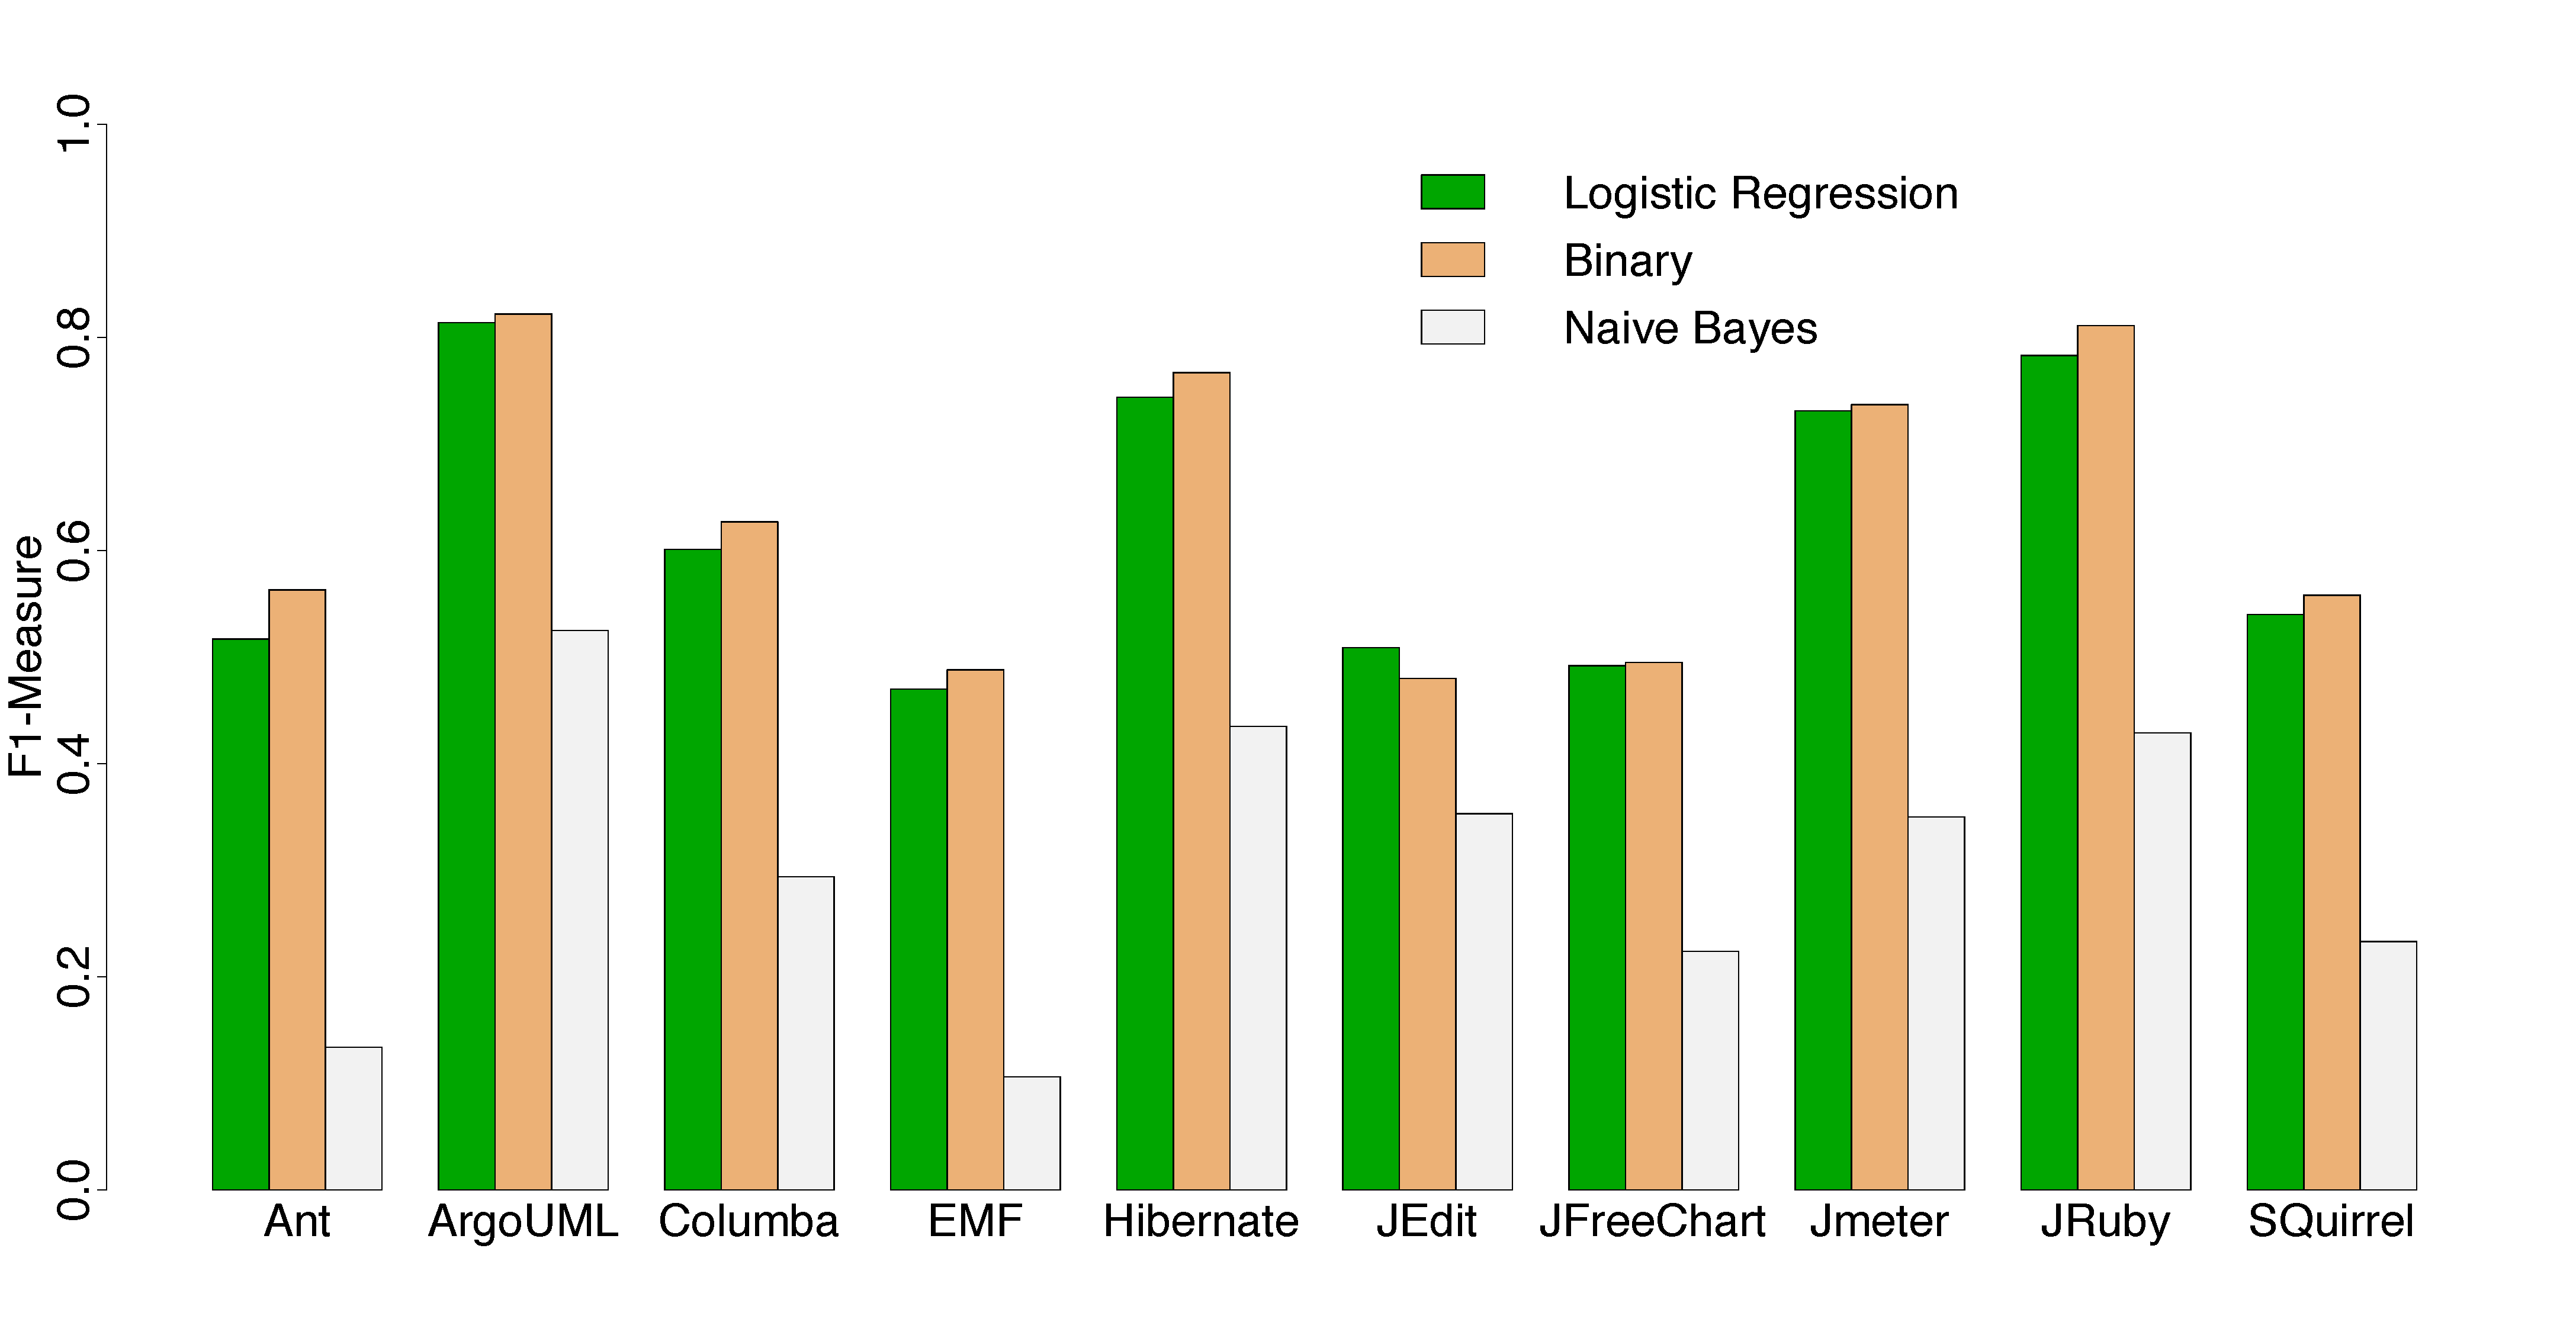
\includegraphics[width=0.48\textwidth]{figures/classifier_algorithms_comparison_design_1.pdf}
  \label{fig:algorithms_comparison_design}}
  \subfigure[Requirement Debt]{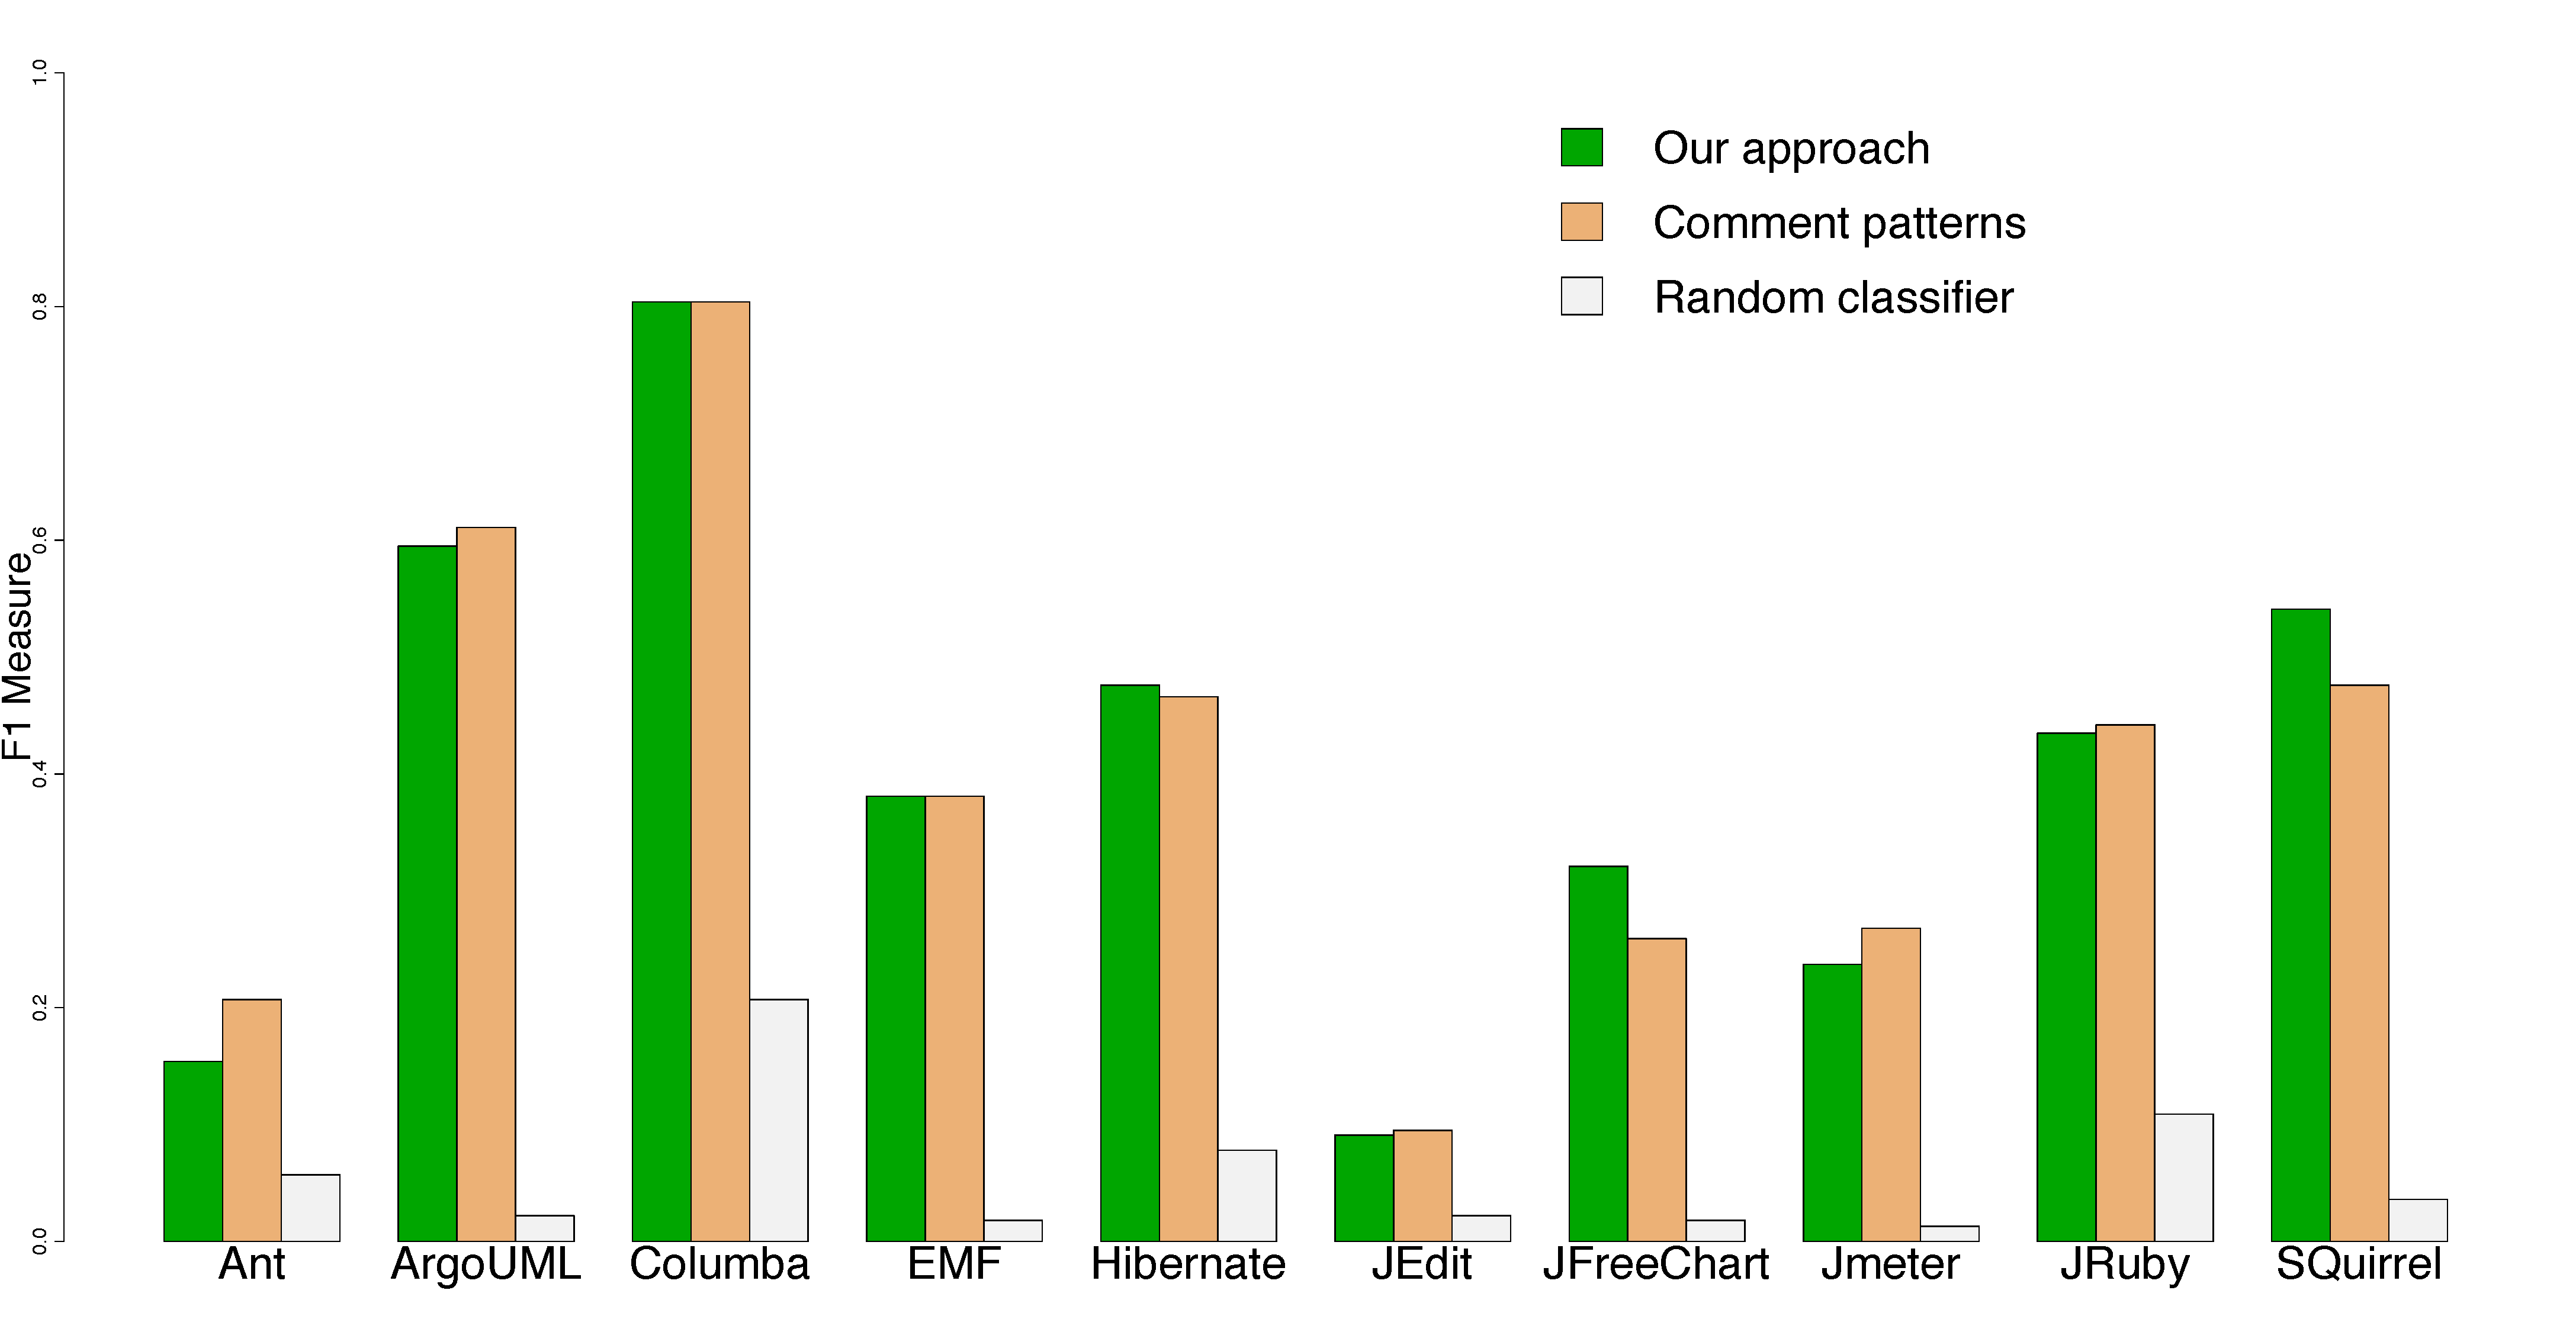
\includegraphics[width=0.48\textwidth]{figures/classifier_algorithms_comparison_implementation_1.pdf}
  \label{fig:algorithms_comparison_requirement}}
  \caption{Underlying Classifier Algorithms Performance Comparison}
  \label{fig:algorithms_comparison}
\end{figure*}

Thus far, we have seen that our NLP-based approach can perform well in classifying \SATD. However, there are some observations that warrant further investigation. For example, when it comes to the different types of \SATD, we find that requirement debt tends to require less training data, which is another interesting point that is worth further investigation. Lastly, when performing our classification, there are a number of underlying classifiers that can be used in the Stanford Classifier, hence we investigate what is the impact of using a different underlying classifier. 
%In this paper we propose an approach to identify \SATD comments using NLP. This tool, once trained correctly, can automatically classify natural language text. We create a training dataset of \SATD comments and analyzed the classification performance across ten open source projects. In RQ1, we show that our approach can outperform the current state-of-the-art in 10 out of 10 projects while identifying design and requirement debt. However, is not clear the reason why our approach was not equally effective across all projects. For example, JEdit has the worst F1 measure of all projects while classifying requirement \SATD.

%\subsection{Investigating Outliers Projects}
%By investigating JEdit comments, we notice two main reasons. First, the project has 10,322 comments. Of those only 14 are requirement \SATD. The data distribution represents a challenge to the classification. Even though the dataset is very unbalanced our precision was 0.125, which compared with the simple (random) baseline precision of 0.001, shows that our approach is still much more useful. Second, most requirement \SATD comments in this project are in the middle of long comments. 
%
%\everton {Since our approach creates a high number of prediction features for \SATD comments and also for comments without technical debt (i.e., positive and negative weight features), long comments have more chances to match a larger set of negative weight features that will lead to the without technical debt classification. Therefore, long comments can generate `noise' that hinders the classification performance of requirement \SATD. Based on our dataset, requirement \SATD comments are short comments having, on average, 81 characters. However, the average size of requirement \SATD comments from JEdit is 149 characters, 1.8$\times$ bigger than the overall average. Assuming that long requirement \SATD comments can be found in more projects that are not analyzed in our work, one can add these hypothetical comments to increment the current training dataset. Nevertheless, based on the projects that were analyzed, we argue that the current training dataset can identify requirement \SATD effectively and long requirement \SATD should be treated as exceptions.} 


% \nikos{I don't get this point}

% \emad{I do not see the point of the 2 paragraphs below}

% \emad{begin: remove} Intuitively we know that each project has its own particularities, and that each group of developers, must often, create a unique way to communicate their concerns with each other. This unique trait of source code comments is inherited from the natural language itself and renders the fully automated prediction of every single \SATD very unlikely. Even when analyzing a old aged project, changes in the context of the application and turnover of developers can reflect changes in the way that source code comments are written. We can notice the impact of these particularities on the detailed performance analysis conducted in RQ3, where we can notice that the addition of more comments can eventually decrease the F1 measure performance.

% For a great portion of \SATD comments there are common traits. Words as `workaround', `hack' are commonly imbued with criticism and the developers sense that this is not the appropriate solution for the problem in hand. However, relying just in these words for the identification of \SATD is not good enough as shown in Figures \ref{fig:f1_measure_comparison_design_debt} and \ref{fig:f1_measure_comparison_requirement_debt}. Therefore, NLP techniques, as proposed in our work, are needed in order to effectively identify \SATD comments.
% \emad{end: remove}



\subsection{Textual Similarity for Design and Requirement Debt}

% tf-idf formula \(tf-idf_{t,d}=tf_{t,d}\times idf_{t} \)
 % \cite{Manning2008book}

In RQ2, we hypothesize that one of the reasons that requirement \SATD comments need less training data is because requirement \SATD comments are more similar to each other than design \SATD comments. Therefore, we set out to measure the intra-similarity between the requirement debt comments and the intra-similarity of design debt comments and compare the two.

% The tf-idf weight is the resulting computation of two other metrics: \textit{term frequency} (tf) and \textit{inverse document frequency} (idf).

We start by calculating the term frequency-inverse document frequency \textit{tf-idf} weight of each design and requirement \SATD comment. The tf is the simple count of occurrences that a term (i.e., word) has in a document (i.e., comment). The idf takes into account the number of documents that the term appears. However, as the name implies, the more one term is repeated across multiple documents the less relevant it is. Therefore, let \textit{N} be the total number of documents in a collection, the inverse document frequency (idf) of a term \textit{t} is defined as follows: \(idf_{t} = log\frac{N}{df_{t}}\). The total tf-idf weight of a document is equals to the sum of each individual term tf-idf weight in the document. Each document is represented by a \textit{document vector} in a \textit{vector space model}. 

Once we have the tf-idf weights for the comments, we calculate the \textit{cosine similarity} between the comments. The Cosine similarity can be viewed as the \textit{dot product} of the normalized versions of two document vectors (i.e., two comments) ~\cite{Manning2008book}. The computation of the cosine distance will vary between 0 to 1, where 0 means that the comments are not similar at all and 1 means that the comments are identical.

%To validate our hypothesis that requirement \SATD comments are more similar to each other than design \SATD comments, we created two separated datasets: one for each type of mentioned \SATD. Then, we apply to each comment the same preprocessing applied to comments in the training and test datasets as described in Subsection \ref{sub:run_the_nlp_classifier}. In addition, we removed English stop words from the comments as the NPL classification tool would do during the process of feature extraction. Then, we calculate the tf-idf weight and the cosine similarity for each comment. 

After calculating the tf-idf we compare each comment to all other comments of the same class and store its cosine similarity. For example, the requirement \SATD dataset contains 757 comments, which will generate a 757$\times$757 matrix (since we compare each comment to all the other comments). Finally, we took the average cosine similarity of each comment of the same type for design and requirement debt and plotted the distribution in Figure \ref{fig:textual_similarity}. Figure \ref{fig:textual_similarity} shows that the median and the upper quartile for requirement \SATD comments are higher than the median and upper quartile for design \SATD. The median for requirement debt comments is 0.018, whereas, the median for design debt comments is 0.011. To ensure that the difference is statistically significant, we perform a Wilcox test to calculate the p-value. The calculated p-value was \textless 2.2e-16 showing that our results is indeed statistically significant (i.e., p \textless 0.001). Considering our findings, our hypothesis is validated, showing that requirement \SATD comments are more similar between them than design \SATD comments are. This may help explain why requirement debt needs a smaller set of textual features to be detected.

\begin{figure}[t]
  \centering
  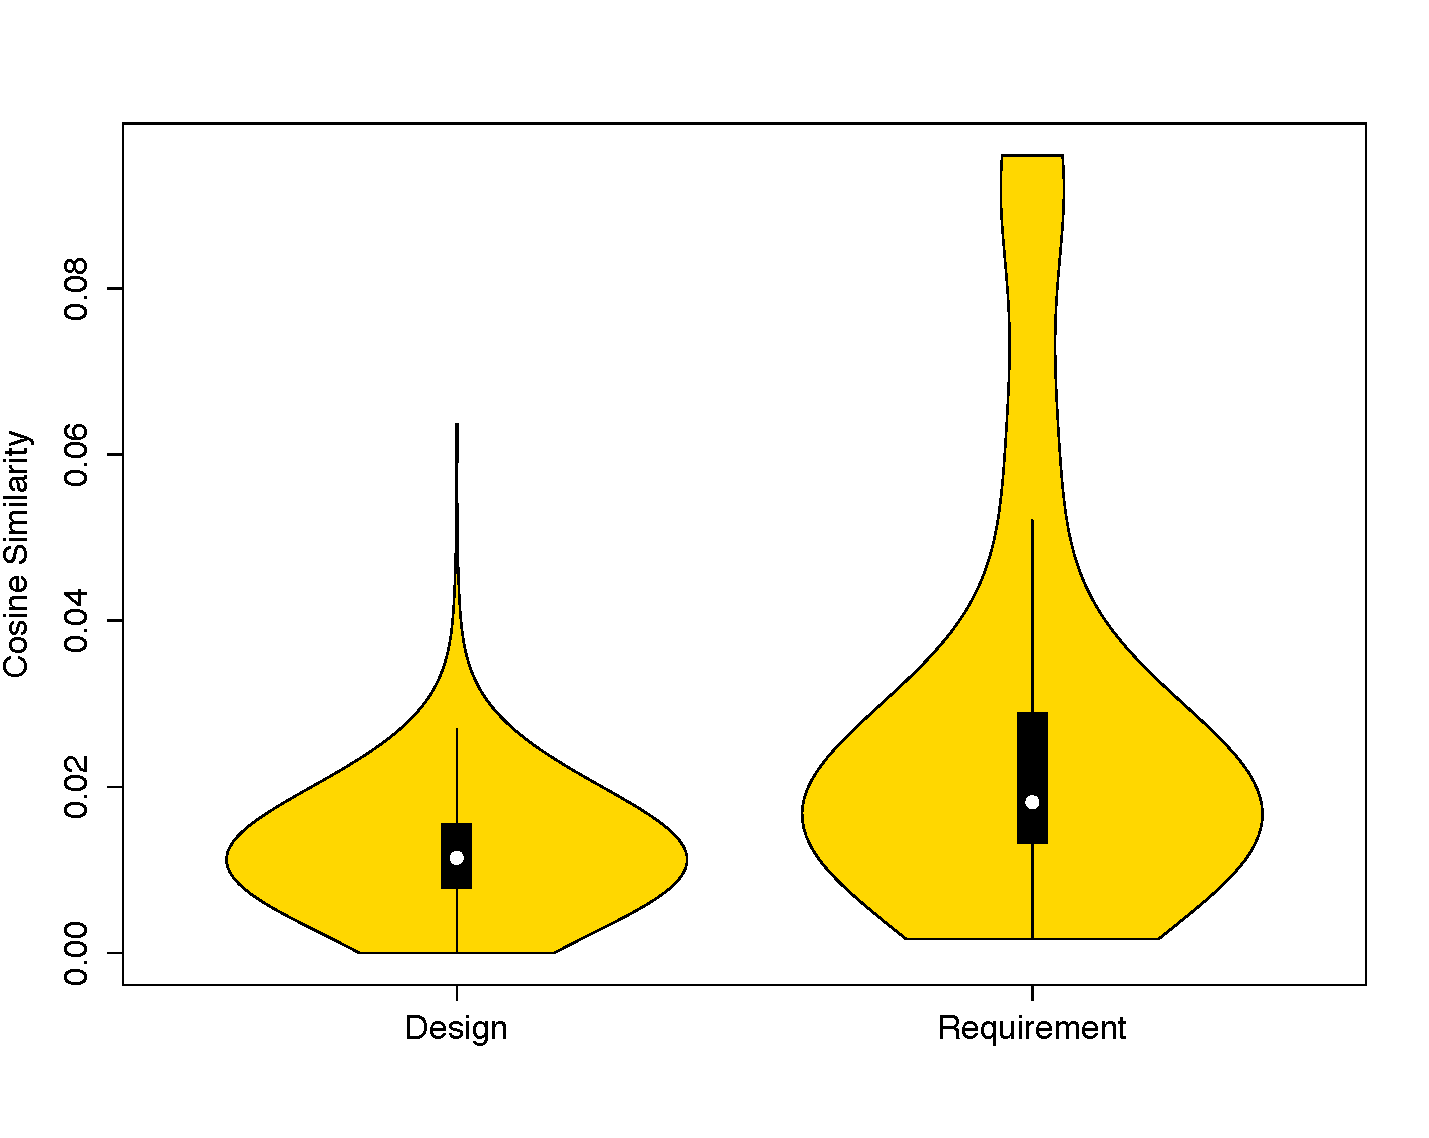
\includegraphics[width = 0.48\textwidth]{figures/textual_similarity_removing_stop_words.pdf}
  \vspace{-3mm}
  \caption{Textual Similarity Between Design and Requirement Debt Comments}
  \label{fig:textual_similarity}
\end{figure}

\subsection{Investigating the Impact of the Underlying Classifier of the NLP Classification}
\label{sec:underlying_classifier}
In our work, all the classification done by the Stanford Classifier used a Logistic Regression classifier. However, the Stanford Classifier can use other classifiers. In order to examine the impact of the underlying classifier on our results, we chose the other two algorithms to execute the classification with, namely the Naive Bayes generative classifier and the Binary classifier.

Figures \ref{fig:algorithms_comparison_design} and \ref{fig:algorithms_comparison_requirement} compare the performance between the three different algorithms. We find that Naive Bayes has the worst average F1-measure of 0.30 and 0.05 for design and requirement technical debt, respectively. Based on our findings, the Naive Bayes algorithm favors recall at the expense of precision. For example, while classifying design debt, the average recall was of 0.84 and precision 0.19. The two other algorithms present more balanced results compared to Naive Bayes, and the difference in performance between them is not as accentuate. The Logistic Regression classifier achieved F1-measures of 0.62 and 0.40, while the binary classifier F1-measures were 0.63 and 0.40, for design and requirement \SATD, respectively. Tables \ref{tbl:improvement_f1measure_between_classifiers_design} and \ref{tbl:improvement_f1measure_between_classifiers_requirement} in the Appendix section provide detailed data for each compared algorithm for all ten projects.

Although the Binary classification has a slightly better performance, for our purpose, the Logistical Regression algorithm provide more insightful features. These features were analyzed and presented in RQ2. 
